
\section{Method}
\label{sec:search_space}

%\subsection{Neural Architecture Search for Large Scale \\Image Classification}




%\subsection{Neural Architecture Search}

%\subsection{Neural Architecture Search with Reinforcement Learning}
Our work makes use of search methods to find good convolutional architectures on a dataset of interest. The main search method we use in this work is the Neural Architecture Search (NAS) framework proposed by~\cite{zoph2017neural}. In NAS, a controller recurrent neural network (RNN) samples child networks with different architectures. The child networks are trained to convergence to obtain some accuracy on a held-out validation set. The resulting accuracies are used to update the controller so that the controller will generate better architectures over time. The controller weights are updated with policy gradient (see Figure~\ref{figure:controller}). %  (see \cite{HuangALS17} for alternate methods that require boosting.)


\begin{figure}[h!]
\begin{center}
%\includegraphics[width=0.6\columnwidth]{figures/newnas.eps}
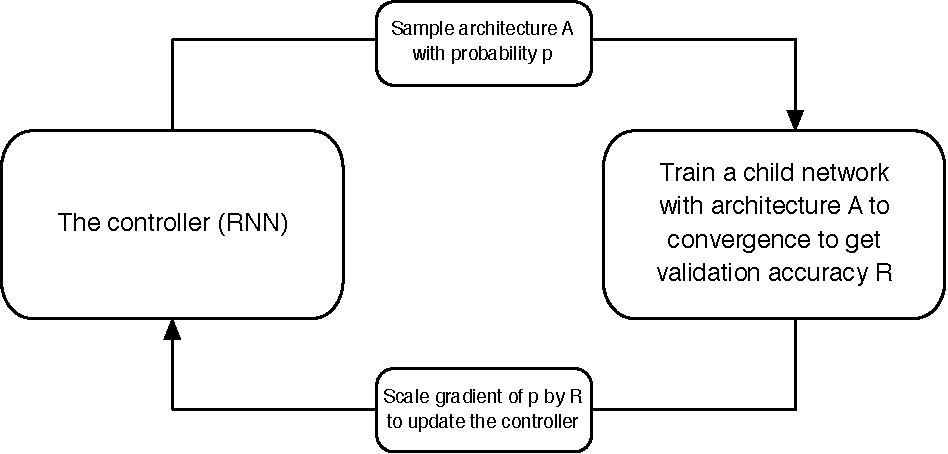
\includegraphics[width=1.0\columnwidth]{NAS-Diagram.pdf}
\caption{Overview of Neural Architecture Search \cite{zoph2017neural}. A controller RNN predicts architecture $A$ from a search space with probability $p$. A child network with architecture $A$ is trained to convergence achieving accuracy $R$. Scale the gradients of $p$ by $R$ to update the RNN controller.}
\label{figure:controller}
\end{center}
\end{figure}
%\todo{Comment: Might it be clearer/more correct to show on the top arrow that you sample a convolutional cell architecture, and then in the right hand box, show that you train a model with 10 sequential copies of this cell architecture?  (Not sure if 10 is the right value, but you get the idea)}

%\subsection{Search Space\label{sec:searchspace}}
%A key element of NAS is to design the search space to generalize across problems of varying complexity and spatial scales. We observed that applying NAS directly to the ImageNet dataset would be very expensive and require months to complete an experiment. However, if the search space is properly constructed, architectural elements can transfer across datasets \cite{zoph2017neural}.


The main contribution of this work is the design of a novel search space, such that the best architecture found on the CIFAR-10 dataset would scale to larger, higher-resolution image datasets across a range of computational settings.
We name this search space \emph{the NASNet search space} as it gives rise to NASNet, the best architecture found in our experiments. One inspiration for the NASNet search space is the realization that architecture engineering with CNNs often identifies 
repeated motifs consisting of combinations of convolutional
filter banks, nonlinearities and a prudent selection of
connections to achieve state-of-the-art results (such as the repeated modules present in the Inception and ResNet models \cite{szegedy2015going,he2015deep,szegedy2016rethinking,szegedy2016inception}). These observations suggest that it may be possible for the controller RNN to predict a generic {\it convolutional cell} expressed in terms of these motifs. This cell can then be stacked in series to handle inputs of arbitrary spatial dimensions and filter depth. 




In our approach, the overall architectures of the convolutional nets are manually predetermined. They are composed of convolutional cells repeated many times where each convolutional cell has the same architecture, but different weights. To easily build scalable architectures for images of any size, we need two types of convolutional cells to serve two main functions when taking in a feature map as input: (1) convolutional cells that return a feature map of the same dimension,  and (2) convolutional cells that return a feature map where the feature map height and width is reduced by a factor of two. We name the first type and second type of convolutional cells  \emph{Normal Cell} and \emph{Reduction Cell} respectively. For the Reduction Cell, we make the initial operation applied to the cell's inputs have a stride of two to reduce the height and width. All of our operations that we consider for building our convolutional cells have an option of striding.

\begin{figure}[t!]
\begin{center}
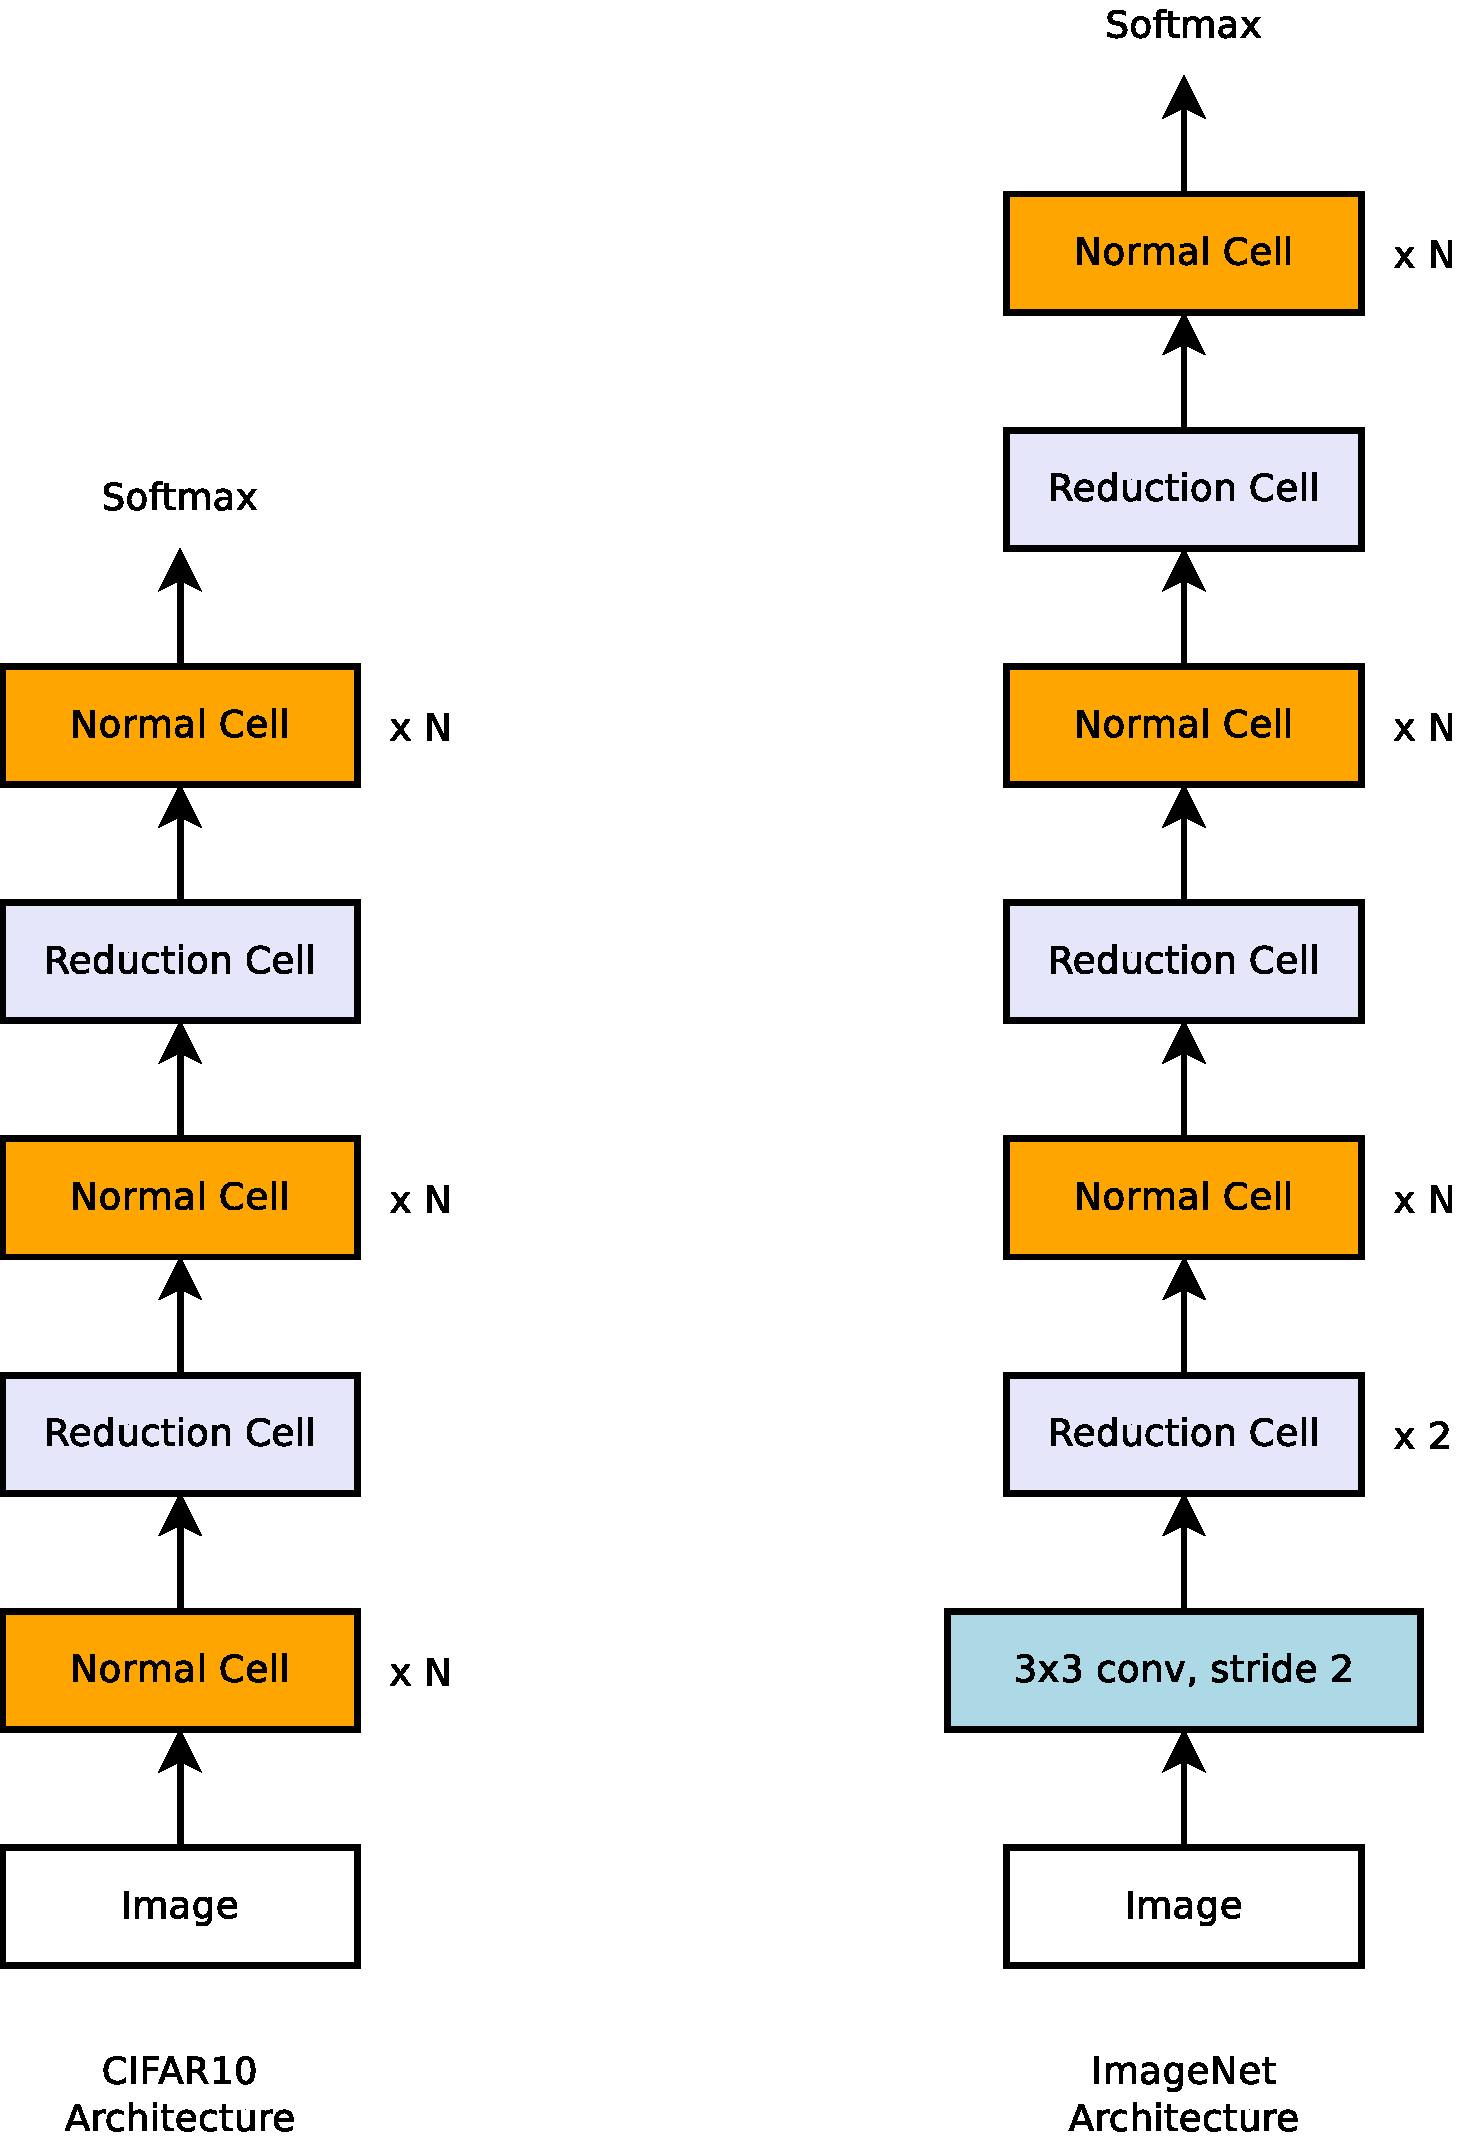
\includegraphics[width=0.7\columnwidth]{main_architecture-eps-converted-to.pdf}
\caption{Scalable architectures for image classification consist of two repeated motifs termed {\it Normal Cell} and {\it Reduction Cell}. This diagram highlights the model architecture for CIFAR-10 and  ImageNet. The choice for the number of times the Normal Cells that gets stacked between reduction cells, $N$, can vary in our experiments.}
%\includegraphics[width=\columnwidth]{figures/Scalable-Architecture.pdf}
%\caption{Scalable architecture for image classification consists of a repeated motif termed a {\it convolutional cell}. The structure of the convolutional cells is shared, but their weights are distinct. The convolutional cell's architecture is predicted by a separate controller RNN. This diagram highlights the model architecture for CIFAR-10 consisting of $N=9$ repeated motifs.}
\label{figure:mainnet}
\end{center}
\end{figure}

Figure~\ref{figure:mainnet} shows our placement of Normal and Reduction Cells for CIFAR-10 and ImageNet. Note on ImageNet we have more Reduction Cells, since the incoming image size is 299x299 compared to 32x32 for CIFAR. The Reduction and Normal Cell could have the same architecture, but we empirically found it beneficial to learn two separate architectures.
We use a common heuristic to double the number of filters in the output whenever the spatial activation size is reduced in order to maintain roughly constant hidden state dimension \cite{krizhevsky2012imagenet,simonyan2014very}.
Importantly,
much like Inception and ResNet models \cite{szegedy2015going,he2015deep,szegedy2016rethinking,szegedy2016inception},
we consider the number of motif repetitions $N$ and the number of initial convolutional filters as free parameters that we tailor to the scale of an image classification problem.




%In terms of CIFAR-10, we stack 9 convolutional cells because it provides a good balance between computational speed and predictive performance (Figure~\ref{figure:mainnet}). At cells 3 and 6 we employ the heuristic to cut the spatial dimensions and increase the filter bank size by a factor of 2. The child network is then trained for just 25 epochs on CIFAR-10. 

%In terms of CIFAR-10, given an architecture, we stack 9 convolutional cells because it provides a good balance between computational speed and predictive performance (Figure~\ref{figure:mainnet}). For cells 3 through 5 in the stack, we double the number of filters compared to the first two cells
%and for cells 6 through 9, we double the number of filters compared to cells 3 through 5.  Cells 3 and 6
%reduce the incoming spatial dimensions of the previous layer activations by a factor of two.
%Each convolutional cell has an option to reducing the spatial dimensions by a factor of two by inserting a stride of 2 after the activations resulting from an initial 1x1 convolution.
%The child network is then trained for just 25 epochs on CIFAR-10. 

%\subsection{Search Space for Convolutional Cells}
%\label{sec:search-space}



%Our search space differs from \cite{zoph2017neural} where the controller needs to predict the entire architecture of the neural networks. 

%In this paper, 
What varies in the convolutional nets is the structures of the Normal and Reduction Cells, which are searched by the controller RNN. 
%Once the overall architecture of the model is defined as shown in Figure \ref{figure:mainnet}, the job of the controller thus becomes predicting the structures of the two convolutional cells: Normal Cell and Reduction Cell.
%which can then be stacked together repeatedly in a fixed repetition pattern for a given task, as shown in Figure \ref{figure:mainnet}. 
%The convolutional cell is inspired by the concept of recurrent cells, where the structure of the cells is independent of the number of time steps in the recurrent network. This is an effective way to decouple the complexity of the cells from the depth of the neural network so that the controller RNN only needs to focus on predicting the structure of the cell. 
The structures of the cells can be searched within a search space defined as follows (see Appendix, Figure \ref{figure:nas-search-space} for schematic). In our search space, each cell receives as input two initial hidden states $h_i$ and $h_{i-1}$ which are the outputs of two cells in previous two lower layers or the input image. The controller RNN recursively predicts the rest of the structure of the convolutional cell, given these two initial hidden states (Figure~\ref{figure:cell}). The predictions of the controller for each cell are grouped into $B$ blocks, where each block has 5 prediction steps made by 5 distinct softmax classifiers corresponding to discrete choices of the elements of a block:

%The outputs of these hidden states represent the initial hidden state the controller RNN may select when predicting the structure of the convolutional cell.
%\todo{Verify paragraph with Barret.} 
%the current cell, and branched into two different hidden states by applying two separate 1x1 convolutions. The outputs of these 1x1 convolutions are the initial hidden states the controller RNN can choose from when predicting the structure of the convolutional cell.

\begin{figure*}[h!]
\begin{center}
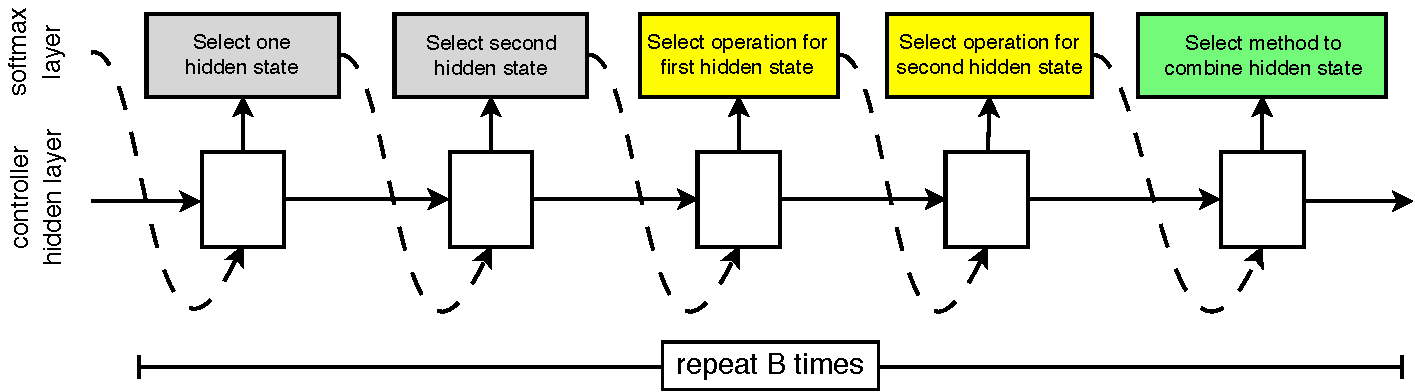
\includegraphics[width=0.7\linewidth]{Figure-2.pdf}
\hfill
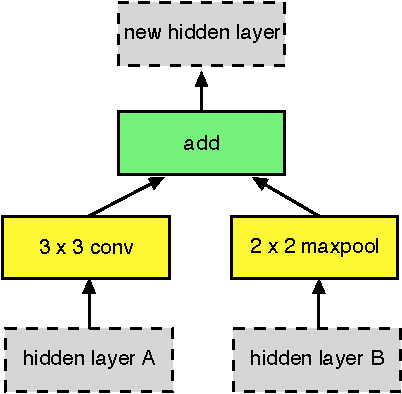
\includegraphics[width=0.2\linewidth]{Figure-2-Part-B.pdf}
\caption{Controller model architecture for recursively constructing one block of a convolutional cell. Each block requires selecting 5 discrete parameters, each of which corresponds to the output of a softmax layer. Example constructed block shown on right. A convolutional cell contains $B$ blocks, hence the controller contains $5B$ softmax layers for
predicting the architecture of a convolutional cell. In our experiments, the number of blocks $B$ is 5.}
\label{figure:cell}
\end{center}
\end{figure*}



\begin{enumerate}[itemindent=0.3cm,label={\bf Step \arabic*.}]
\footnotesize
\item Select a hidden state from $h_i, h_{i-1}$ or from the set of hidden states created in previous blocks.
\item Select a second hidden state from the same options as in Step 1.
\item Select an operation to apply to the hidden state selected in Step 1. 
\item Select an operation to apply to the hidden state selected in Step 2.
\item Select a method to combine the outputs of Step 3 and 4 to create a new hidden state.
\end{enumerate}
The algorithm appends the newly-created hidden state to the set of existing hidden states as a potential input in subsequent blocks. The controller RNN repeats the above 5 prediction steps $B$ times corresponding to the $B$ blocks in a convolutional cell. In our experiments, selecting $B=5$ provides good results, although we have not exhaustively searched this space due to computational limitations. 

In steps 3 and 4, the controller RNN selects an operation to apply to the hidden states. We collected the following set of operations based on their prevalence in the CNN literature:

\begin{table}[H]
\footnotesize
\setlength{\tabcolsep}{0.5em} % for the horizontal padding
\centering
\def\arraystretch{1.0}
\begin{tabular}{ll}
$\bullet\;$ identity & $\bullet\;$ 1x3 then 3x1 convolution \\
$\bullet\;$ 1x7 then 7x1 convolution & $\bullet\;$ 3x3 dilated convolution \\
$\bullet\;$ 3x3 average pooling & $\bullet\;$ 3x3 max pooling \\
$\bullet\;$ 5x5 max pooling & $\bullet\;$ 7x7 max pooling \\
$\bullet\;$ 1x1 convolution & $\bullet\;$ 3x3 convolution \\
$\bullet\;$ 3x3 depthwise-separable conv & $\bullet\;$ 5x5 depthwise-seperable conv \\
$\bullet\;$ 7x7 depthwise-separable conv \\
\end{tabular}
\end{table}
%In our experiments, we apply each separable operation twice during the execution of the child model, once that operation is selected by the controller.

In step 5 the controller RNN selects a method to combine the two hidden states, either (1) element-wise addition between two hidden states or (2) concatenation between two hidden states along the filter dimension.
Finally, all of the unused hidden states generated in the convolutional cell are concatenated together in depth to provide the final cell output.


To allow the controller RNN to predict both Normal Cell and Reduction Cell, we simply make the controller have $2\times 5B$ predictions in total, where the first $5B$ predictions are for the Normal Cell and the second $5B$ predictions are for the Reduction Cell.

Finally, our work makes use of the reinforcement learning proposal in NAS~\cite{zoph2017neural}; however, it is also possible to use random search to search for architectures in the NASNet search space. In random search, instead of sampling the decisions from the softmax classifiers in the controller RNN, we can sample the decisions from the uniform distribution. In our experiments, we find that random search is slightly worse than reinforcement learning on the CIFAR-10 dataset. Although there is value in using reinforcement learning, the gap is smaller than what is found in the original work of~\cite{zoph2017neural}. This result suggests that 1) the NASNet search space is  well-constructed such that random search can perform reasonably well and 2) random search is a difficult baseline to beat. We will compare reinforcement learning against random search in Section~\ref{sec:random_search}.



%\textcolor{red}{QVL: Barret, we should talk about the initial hidden states given to the model.}
%\textcolor{red}{barretzoph: Quoc what do you think about the description below?}
%After all of predictions have been made for the convolutional cell, all of the unused hidden states that have been created are concatenated together. This final hidden state is the output of the convolutional cell.
%\todo{Verify with Barret that addition operation is not performed anywhere the results presented.}

%In the experiments below, we explore each combination method.

% vrv: Most of this is no longer true, commenting out.  It is also described below.
% We also use a parameter-server scheme where we have a parameter server to store the shared parameters for a number of controller replicas. Each controller replica samples a number of different child architectures that are trained in parallel. The gradients according to the results of that minibatch of generated architectures at convergence are collected and sent to the parameter server in order to update the weights across all controller replicas. In our implementation, convergence of each child network is reached when its training exceeds a certain number of epochs.
